\newpage

\section{In-depth study} % (fold)
\label{sec:in_depth_study}

\subsection{The tables} % (fold)
\label{sub:the_tables}

\subsubsection{General tables} % (fold)
\label{ssub:general_tables}
Tables are the only data structure "container" integrated in Lua.
 They are associative arrays  which associates a key (reference or index) with a value in the form of a field (set) of key/value pairs. Moreover, tables have no fixed size and can grow based on our need dynamically.

Tables are created using table constructors,  the simplest of which is the use of braces, e.g. \{ \}. This defines an empty table.

\begin{mybox}
\begin{Verbatim}
  F = {"banana", "apple", "cherry"}
\end{Verbatim}
\end{mybox}


print(F[2]) --> pomme


qui peut être également définit par

\begin{mybox}
\begin{Verbatim}
   FR = {[1] = "banana", [3] = "cherry", [2] = "apple"}
\end{Verbatim}
\end{mybox}


print(FR[3]) --> cherry

FR[4]="orange"

\begin{mybox}
\begin{Verbatim}
   print(#FR)
   -- I for Index
   for I,V in ipairs(FR) do
      print(I,V)
   end 
\end{Verbatim}
\end{mybox}

1 banana\\
2 apple\\
3 cherry\\
4 orange\\

\begin{mybox}
\begin{Verbatim}
C = {["banana"] = "yellow" , ["apple"] = "green" , ["cherry"] = "red" }
C.orange = "orange"
\end{Verbatim}
\end{mybox}

\begin{mybox}
\begin{Verbatim}
   for K,V in pairs (C) do
      print(K,V)
   end
\end{Verbatim}
\end{mybox}

banana = yellow
cherry = red
orange = orange
apple  = green
% subsection the_tables (end)

Another useful feature is the ability to create a table to store an unknown number of function parameters, for example:

\begin{mybox}
\begin{Verbatim}
  function ReturnTable (...)
    return table.pack (...) 
  end 
\end{Verbatim}
\end{mybox}

\begin{mybox}
\begin{Verbatim}
  function ParamToTable (...)
    mytab =  ReturnTable(...)
      for i=1,mytab.n do
        print(mytab[i])
      end
  end
  ParamToTable("cherry","apple","orange")  
\end{Verbatim}
\end{mybox}


Using tables with table[key] syntax:

|C["banana"] and F[1]  |

But with  string constants as keys we have the sugar syntax:
C.banana but this syntax does not accept numbers.

It's possible to erase a key/value pair from a table, with :

\begin{mybox}
\begin{Verbatim}
  C.banana = nil 
\end{Verbatim}
\end{mybox}
% subsubsection general_tables (end)

\subsubsection{Table z} % (fold)
\label{ssub:table_z}
This is the most important table in the package. It stores all points and enables them to be transferred to \TIKZ{}.

It is defined with |z = {}|, then each time we write

\begin{mybox}
   | z.name = point : new (a , b)|
\end{mybox}

a point object is stored in the table. The key is |name|, the value is an object. We have seen that |z.name.re = a| and that |z.name.im = b|.

However, the elements of this table have essential properties.

For example, if you wish to display an element, then |tex.print(tostring(z.name)) = a+ib| the |tostring| operation displays the affix corresponding to the point.

In addition, we'll see that it's possible to perform operations with the elements of the |z| table.
% subsubsection table_z (end)

\subsection{Transfers} % (fold)
\label{sub:transfers}

We've seen (sous-section \ref{ssub:points_transfer}) that the macro \Imacro{tkzGetNodes} transfers point coordinates to \TIKZ. Let's take a closer look at this macro:

\vspace*{1em}

\begin{mybox}
\begin{Verbatim}
\def\tkzGetNodes{\directlua{%
   for K,V in pairs(z) do
      local K,n,sd,ft
      n = string.len(KS)
      if n >1 then
      _,_,ft, sd = string.find( K , "(.+)(.)" )  
     if sd == "p" then   K=ft.."'" end  
       end    
  tex.print("\\coordinate ("..K..") at ("..V.re..","..V.im..") ;\\\\")
end}
}
\end{Verbatim}
\end{mybox}

It consists mainly of a loop. The variables used are K (for keys) and V (for Values). To take pairs (key/value) from the |z| table, use the |pairs| function. K becomes the name of a node whose coordinates are |V.re| and |V.im|. Meanwhile, we search for keys with more than one symbol ending in |p|, in order to associate them with the symbol "'" valid in \TIKZ{}.
% subsection transfers (end)

\subsection{Complex numbers library and point} % (fold)
\label{sub:complex_numbers}

Unless you want to create your own functions, you won't need to know and use complex numbers. However, in some cases it may be useful to implement some of their properties.


|z.A =  point : new (1,2 )| and \ |z.B = point : new (1,-1)| define two affixes which are $z_A = 1+2i$ and $z_B = 1-i$. Note the difference in notations |z.A| and $z_A$ for two distinct entities: a Lua object and an affix. 

\vspace{1em}
If you want to use only complex numbers then you must choose the following syntax :|za =point (1,2)|.
The difference between |z.A = point : new (1,2)| and |za = point (1,2)| is that the first function takes into account the scale. If |scale = 2| then $z_A = 2+4i$. In addition, the object referenced by A is stored in table |z| and not za.

 The notation may come as a surprise, as I used the term "point". The aim here was not to create a complete library on complex numbers, but to be able to use their main properties in relation to points. I didn't want to have two different levels, and since a unique connection can be established between the points of the plane and the complexes, I decided not to mention the complex numbers! But they are there.


\bgroup
\catcode`_=12
\small

\begin{minipage}{\textwidth}
\captionof{table}{Point or complex metamethods.}\label{complex:meta}
\begin{tabular}{lll}
  \toprule
  \textbf{Metamethods} & \textbf{Application} \\
  \midrule
\_\_\Immeth{point}{add(z1,z2)}   & |z.a + z.b| & affix \\
\_\_\Immeth{point}{sub(z1,z2)}   & |z.a - z.b| & affix\\
\_\_\Immeth{point}{unm(z)}       & |- z.a| & affix\\
\_\_\Immeth{point}{mul(z1,z2)}   & |z.a * z.b|  &  affix\\
\_\_\Immeth{point}{concat(z1,z2)}& |z.a .. z.b| & dot product  = real number \footnote{If $O$ is the origin of the complex plan, then we get the dot product of the vectors $\overrightarrow{Oa}$ and $\overrightarrow{Ob}$} \\
\_\_\Immeth{point}{pow(z1,z2)}  & |z.a ^ z.b| & determinant = real number\\
\_\_\Immeth{point}{div(z1,z2)}  & |z.a / z.b|   &   affix     \\
\_\_\Immeth{point}{tostring(z)} & tex.print(tostring(z)) & displays the affix   \\
\_\_\Immeth{point}{tonumber(z)}   & tonumber(z) & affix or nil\\
\_\_\Immeth{point}{eq(z1,z2)}    &  eq (z.a,z.b) & boolean\\
\bottomrule
\end{tabular}
\end{minipage}
\egroup

\bgroup
\catcode`_=12
\small
\begin{minipage}{\textwidth}
\captionof{table}{Point (complex) class methods.}\label{complex:met}
\begin{tabular}{lll}
  \toprule
\textbf{Methods} & \textbf{Application}\\
\midrule
\Imeth{point}{conj(z)}  & |z.a : conj()|   & affix (conjugate) \\
\Imeth{point}{mod(z)}   & |z.a : mod()|    & real number = modulus  |z.a|\\
\Imeth{point}{abs (z)}  & |z.a : abs()|    & real number = modulus \\
\Imeth{point}{norm (z)} & |z.a : norm()|   & norm  (real number  ) \\
\Imeth{point}{arg (z)} & |z.a : arg()|    & real number = argument of z.a (in rad)\\
\Imeth{point}{get(z)}   & |z.a : get()|    & re and im (two real numbers  )  \\
\Imeth{point}{sqrt(z)} & |z.a : sqrt()|   & affix  \\
\bottomrule
\end{tabular}
\end{minipage}
\egroup

\vspace{1em}
The class is provided with two specific metamethods.

\begin{itemize}
   \item Since concatenation makes little sense here, the operation associated with |..| is the scalar or dot product. If |z1 = a+ib| and |z2 = c+id| then

   |z1..z2 = (a+ib) .. (c+id) = (a+ib) (c-id) = ac+bd + i(bc-ad) |

   There's also a mathematical function, |dot_product|, which takes three arguments. See example \ref{sub:dot_or_scalar_product}


   \item With the same idea, the operation associated with |^| is the determinant i.e.

   |z1 ^ z2 = (a+ib) ^ (c+id) = ad - bc  From  (a-ib) (c+id) = ac+bd + i(ad - bc)| we take the imaginary part.

\end{itemize}

\subsubsection{Example of complex use} % (fold)
\label{ssub:example_of_complex_use}
Let |za = math.cos(a) + i math.sin(a)| . 
This is obtained from the library by writing 

\begin{mybox}
   |za = point(math.cos(a),math.sin(a))|.
\end{mybox}

Then |z.B = z.A * za| describes a rotation of point A by an angle |a|.

\begin{minipage}{.6\textwidth}
   \begin{Verbatim}
      \begin{tkzelements}
         z.O = point : new (0,0)
         z.A = point : new (1,2)
         a = math.pi/6
         za = point(math.cos(a),math.sin(a))
         z.B = z.A * za
      \end{tkzelements}
      \begin{tikzpicture}
      \tkzGetNodes
      \tkzDrawPoints(O,A,B)
      \tkzDrawArc[->,delta=0](O,A)(B)
      \tkzDrawSegments[dashed](O,A O,B)
      \tkzLabelAngle(A,O,B){$\pi/6$}
      \end{tikzpicture}
   \end{Verbatim}
\end{minipage}
\begin{minipage}{.6\textwidth}
\begin{tkzelements}
   scale=2
   z.O = point : new (0,0)
   z.A = point : new (1,2)
   a = math.pi/6
   za = point(math.cos(a),math.sin(a))
   z.B = z.A * za
\end{tkzelements}
\begin{tikzpicture}
\tkzGetNodes
\tkzDrawPoints(O,A,B)
\tkzDrawArc[->,delta=0,thick](O,A)(B)
\tkzDrawSegments[dashed](O,A O,B)
\tkzLabelAngle(A,O,B){$\pi/6$}
\end{tikzpicture}
\end{minipage}
% subsubsection example_of_complex_use (end)

\subsubsection{Point operations (complex)} % (fold)
\label{ssub:point_operations_complex}

\begin{minipage}{.5\textwidth}
\begin{Verbatim}
\begin{tkzelements}
   z.o  = point: new(0,0)
   z.a  = point: new(1,-1)
   z.b  = point: new(2,1)
   z.bp = -z.b
   z.c  = z.a + z.b
   z.d  = z.a - z.b
   z.e  = z.a * z.b
    z.f  = z.a / z.b
    z.ap = point.conj (z.a)
    -- = z.a : conj ()
   z.g = z.b* point(math.cos(math.pi/2),
                   math.sin(math.pi/2))
\end{tkzelements}

\hspace*{\fill}   
\begin{tikzpicture}
 \tkzGetNodes
 \tkzInit[xmin=-2,xmax=3,ymin=-2,ymax=3]
 \tkzGrid
 \tkzDrawSegments(o,a o,b o,c o,e o,b' o,f o,g)
 \tkzDrawSegments[red](a,c b,c b',d a,d)
 \tkzDrawPoints(a,...,g,o,a',b')
 \tkzLabelPoints(o,a,b,c,d,e,f,g,a',b')
\end{tikzpicture}
\end{Verbatim}
   \end{minipage}
\begin{minipage}{.5\textwidth}
 \begin{tkzelements}
 z.o  = point: new(0,0)
 z.a  = point: new(1,-1)
 z.b  = point: new(2,1)
 z.bp = -z.b
 z.c  = z.a + z.b
 z.d  = z.a - z.b
 z.e  = z.a * z.b
  z.f  = z.a / z.b
  z.ap = point.conj (z.a)
  -- = z.a : conj ()
 z.g = z.b* point(math.cos(math.pi/2),math.sin(math.pi/2))
\end{tkzelements}
   
\hspace*{\fill}   
\begin{tikzpicture}
         \tkzGetNodes
         \tkzInit[xmin=-2,xmax=3,ymin=-2,ymax=3]
          \tkzGrid
         \tkzDrawSegments(o,a o,b o,c o,e o,b' o,f o,g)
         \tkzDrawSegments[red](a,c b,c b',d a,d)
         \tkzDrawPoints(a,...,g,o,a',b')
         \tkzLabelPoints(o,a,b,c,d,e,f,g,a',b')
\end{tikzpicture}
\end{minipage}
% subsubsection point_operations_complex (end)
% subsection complex_numbers (end)


\subsection{Barycenter} % (fold)
\label{sub:barycenter}

\begin{minipage}{.8\textwidth}
   Here's the definition of the barycenter, which is used some forty times in the package.
|table.pack| builds a table from a list. \\
|tp.n| gives the number of pairs. \\
|tp[i][1]| is an affix and |tp[i][2]| the associated weight (real value). 5se the example.
         
\begin{Verbatim}
   function barycenter_ (...)
   local tp = table.pack(...)
   local i
   local sum = 0
   local weight=0
   for i=1,tp.n do
      sum = sum + tp[i][1]*tp[i][2]
      weight = weight + tp[i][2]
   end
   return sum/weight
   end
\end{Verbatim}
\end{minipage}

\vspace{1em}   
\subsubsection{Using the barycentre} % (fold)
\label{ssub:using_the_barycentre}

\begin{minipage}{.5\textwidth}
\begin{Verbatim}
\begin{tkzelements}
 z.A =  point: new (1,0)
 z.B =  point: new (5,-1)
 z.C =  point: new (2,5)
 z.G =  barycenter ({z.A,3},{z.B,1},{z.C,1})
\end{tkzelements}
    
\begin{tikzpicture}
\tkzGetNodes
\tkzDrawPolygon(A,B,C)
\tkzDrawPoints(A,B,C,G)
\end{tikzpicture}
\end{Verbatim}
\end{minipage}
\begin{minipage}{.5\textwidth}\begin{tkzelements}
 z.A =  point: new (1,0)
 z.B =  point: new (5,-1)
 z.C =  point: new (2,5)
 z.G =  barycenter ({z.A,3},{z.B,1},{z.C,1})
\end{tkzelements}
 \hspace{\fill}  
\begin{tikzpicture}
\tkzGetNodes
\tkzDrawPolygon(A,B,C)
\tkzDrawPoints(A,B,C,G)
\end{tikzpicture}
\end{minipage}
% subsubsection using_the_barycentre (end)

\subsubsection{Incenter of a triangle} % (fold)
\label{ssub:incenter_of_a_triangle}
The calculation of the weights ka, kb and kc is precise, and the result obtained with the barycenter is excellent. Note the presence of the underscore \_ for certain functions. These functions are internal (developer). Each external (user) function is associated with its internal counterpart.

Here's how to determine the center of the inscribed circle of a triangle:
\begin{mybox}
\begin{Verbatim}
   function in_center_ ( a,b,c )
      local ka = point.abs (b-c)
      local kc = point.abs (b-a)
      local kb = point.abs (c-a)
      return    barycenter_ ( {a,ka} , {b,kb} , {c,kc} )
   end \end{Verbatim}
\end{mybox}

% subsubsection incenter_of_a_triangle (end)  
% subsection barycenter (end)

\subsection{Loop and table notation} % (fold)
\label{sub:loop_and_table_notation}
The problem encountered in this example stems from the notation of the point names. Since it's not possible to write in simplified form, we have to resort to table[key] notation.

\begin{minipage}{.5\textwidth}
\begin{Verbatim}
\begin{tkzelements}
  local r  = 3
  z.O      = point : new (0,0)
  max      = 100
  for i    = 1,max 
  do 
     z["A_"..i] = point : polar(r,2*i*math.pi/max)
  end
  a = math.deg(get_angle (z.O,z.A_1,z.A_2))
\end{tkzelements}
\end{Verbatim}
\end{minipage}
\begin{minipage}{.5\textwidth}
\begin{tkzelements}
  local r  = 3
  z.O      = point : new (0,0)
  max      = 100
  for i    = 1,max 
  do 
     z["A_"..i] = point : polar(r,2*i*math.pi/max)
  end
  a = math.deg(get_angle (z.O,z.A_1,z.A_2))
\end{tkzelements}
\hspace{\fill}
\begin{tikzpicture}
\pgfkeys{/pgf/number format/.cd,use comma}
\let\pmpn\pgfmathprintnumber
\tkzGetNodes
\tkzDrawPolygon[cyan](A_1,A_...,A_\tkzUseLua{max})
\tkzDrawCircle[red](O,A_1)
\tkzDrawPoints[color=black](A_1,A_...,A_\tkzUseLua{max},O)
\tkzDrawSegments(O,A_1 O,A_2)
\tkzMarkAngle[size=2](A_1,O,A_2)
\tkzLabelAngle[pos=3.4](A_1,O,A_2){$\pmpn{\tkzUseLua{a}}^\circ$}
\end{tikzpicture}
\end{minipage}

% subsection loop_and_table_notation (end)

\subsection{In\_out method} % (fold)
\label{sub:in_out_method}

This function can be used for the following objects
\begin{itemize}
   \item line
   \item circle 
   \item triangle
   \item ellipse
\end{itemize}
 The disk object doesn't exist, so with |in\_out\_disk| it's possible to determine whether a point is in a disk.

\subsubsection{In\_out for a line} % (fold)
\label{ssub:in_out_for_a_line}

\begin{mybox}
\begin{Verbatim}
  function line: in_out (pt)
  local sc,epsilon
  epsilon = 10^(-12)
  sc = math.abs ((pt-self.pa)^(pt-self.pb))
  if sc <= epsilon
     then 
        return true
     else 
        return false 
     end
  end 
\end{Verbatim}
\end{mybox}

The \tkzNamePack{ifthen} package is required for the code below.

\begin{minipage}{.5\textwidth}
\begin{Verbatim}
\begin{tkzelements}
z.A     = point: new (0,0)
z.B     = point: new (1,2)
z.X     = point: new (2,4.000)
z.Y     = point: new (2,4.1)
L.AB = line :  new (z.A,z.B)
if L.AB : in_out (z.X)
  then
   inline = true  k = (z.X-z.A)/(z.B-z.A)
  else
   inline = false
  end
 inline_bis = L.AB : in_out (z.Y)
\end{tkzelements}

\begin{tikzpicture}
\tkzGetNodes
\tkzDrawPoints(A,B,X,Y)
\tkzLabelPoints(A,B,X)
\tkzLabelPoints[left](Y)
\ifthenelse{\equal{\tkzUseLua{inline}}{true}}{
   \tkzDrawSegment[red](A,B)
   \tkzLabelSegment(A,B){AX/AB = $\tkzUseLua{k}$}}{%
   \tkzDrawSegment[blue](A,B)}
\ifthenelse{\equal{\tkzUseLua{inline_bis}}{false}}{%
 \tkzDrawSegment[green](B,Y)}{}
\end{tikzpicture}
\end{Verbatim}
\end{minipage}
\begin{minipage}{.5\textwidth}
   \begin{tkzelements}
z.A     = point: new (0,0)
z.B     = point: new (1,2)
z.X     = point: new (2,4.000)
z.Y     = point: new (2,4.1)
L.AB = line :  new (z.A,z.B)
if L.AB : in_out (z.X)
  then
   inline = true  k = (z.X-z.A)/(z.B-z.A)
  else
   inline = false
  end
 inline_bis = L.AB : in_out (z.Y)
\end{tkzelements}
\hspace{\fill}
\begin{tikzpicture}
\tkzGetNodes
\tkzDrawPoints(A,B,X,Y)
\tkzLabelPoints(A,B,X)
\tkzLabelPoints[left](Y)
\ifthenelse{\equal{\tkzUseLua{inline}}{true}}{
   \tkzDrawSegment[red](A,B)
   \tkzLabelSegment(A,B){AX/AB = $\tkzUseLua{k}$}}{%
   \tkzDrawSegment[blue](A,B)}
\ifthenelse{\equal{\tkzUseLua{inline_bis}}{false}}{
\tkzDrawSegment[green](B,Y)}{}
\end{tikzpicture}
\end{minipage}
% subsubsection in_out_for_a_line (end) 
% subsection in_out_method (end)


\subsection{Determinant and dot product} % (fold)
\label{sub:determinant_et_produit_scalaire}

\subsubsection{Determinant} % (fold)
\label{ssub:determinant}

We've just seen how to use |^| to obtain the determinant associated with two vectors. 

\Imeth{line}{in\_out}  is simply a copy of  \Imeth{math}{islinear} .

Here's the definition and transformation of the power of a complex number.

\begin{Verbatim}
   -- determinant  is '^'   ad - bc
   function point.__pow(z1,z2)
       local z
       z = point.conj(z1) * z2   -- (a-ib) (c+id) = ac+bd + i(ad - bc)
      return z.im
   end
\end{Verbatim}
% subsubsection determinant (end)


\subsubsection{Dot product} % (fold)
\label{ssub:scalar_product}

Here's the definition of the dot product between two affixes and the concatenation transformation. 

\begin{Verbatim}
-- dot product is '..'         result ac + bd
function point.__concat(z1,z2)
    local z
    z = z1 * point.conj(z2)         -- (a+ib) (c-id) = ac+bd + i(bc-ad) 
  return z.re
end
\end{Verbatim}
% subsubsection scalar_product (end)



\subsubsection{Dot product: orthogonality test } % (fold)
\label{ssub:scalar_product_orthogonality_test}

Here's a function  \Imeth{math}{isortho} to test orthogonality between two vectors.

\begin{Verbatim}
function isortho (z1,z2,z3)
   local epsilon
   local dp
   epsilon = 10^(-8)
   dp = (z2-z1) .. (z3-z1)
   if math.abs(dp) < epsilon 
    then 
        return true
    else 
        return false
    end
end
\end{Verbatim}
% subsubsection scalar_product_orthogonality_test (end)


\subsubsection{Dot product: projection} % (fold)
\label{ssub:scalar_product_projection}

The projection of a point onto a straight line is a fundamental function, and its definition is as follows:

\begin{Verbatim}
function projection_ ( pa,pb,pt )
   local v
   local z
   if aligned ( pa,pb,pt ) then
   return pt
   else
    v = pb - pa
    z = ((pt - pa)..v)/(point.norm(v)) -- .. dot product
   return pa + z * v  
   end
end
\end{Verbatim}

The function  \Imeth{math}{aligned} is equivalent to  \Imeth{math}{islinear}  but does not use a determinant. It will be replaced in a future version.

% subsubsection scalar_product_projection (end)
% subsection determinant_et_produit_scalaire (end)

\subsection{Point method} % (fold)
\label{sub:point_method}

The point  method is a method for many objects: 
\begin{itemize}
 \item line ,
 \item circle,
 \item ellipse,
 \item triangle.
\end{itemize}

You obtain a point on the object by entering a real number between 0 and 1. 

\begin{minipage}{.5\textwidth}
\begin{Verbatim}
\begin{tkzelements}
   z.A   = point : new ( 0 , 0 ) 
   z.B   = point : new ( 4 , 2 ) 
   z.C   = point : new ( 1 , 3 )
   L.AB  = line : new (z.A,z.B)
   C.AB  = circle  : new (z.A,z.B) 
   T.ABC = triangle  : new  (z.A,z.B,z.C)
   z.I   = L.AB : point (0.5)
   z.J   = C.AB : point (0.5)
   z.K   = T.ABC : point (0.5)
\end{tkzelements}
\begin{tikzpicture}
   \tkzGetNodes
   \tkzDrawLine(A,B)
   \tkzDrawCircle(A,B)
   \tkzDrawPolygon(A,B,C)
   \tkzDrawPoints(A,B,C,I,J,K)
\end{tikzpicture}
\end{Verbatim}
\end{minipage}
\hspace{\fill}
\begin{minipage}{.5\textwidth}
\begin{tkzelements}
   scale =.75
   z.A   = point : new ( 0 , 0 ) 
   z.B   = point : new ( 4 , 2 ) 
   z.C   = point : new ( 1 , 3 )
   L.AB  = line : new (z.A,z.B)
   C.AB  = circle  : new (z.A,z.B) 
   T.ABC = triangle  : new  (z.A,z.B,z.C)
   z.I   = L.AB : point (0.5)
   z.J   = C.AB : point (0.5)
   z.K   = T.ABC : point (0.5)
\end{tkzelements}
\begin{tikzpicture}
\tkzGetNodes
\tkzDrawLine(A,B)
\tkzDrawCircle(A,B)
\tkzDrawPolygon(A,B,C)
\tkzDrawPoints(A,B,C,I,J,K)
\end{tikzpicture}
\end{minipage}

% subsection point_method (end)

\subsection{Behind the objects} % (fold)
\label{sub:behind_the_objects}

Before introducing objects, I only used functions whose parameters were points (comlexes). 

For example, |z.m = midpoint_ (z.a,z.b)| defines the midpoint of points $a$ and $b$. With objects, first define the line/sgment |L.ab| and then obtain the middle with |z.m = L.ab.mid|.

I've kept the functions (which I'll call "primary") whose only arguments are points. They are distinguished from the others by a terminal underscore. In fact, all (almost) object-related functions depend on a primary function.

We've just seen the case of the midpoint of a point, so let's look at two other cases:

\begin{itemize}
   \item Rotation around a point. |c| is the center of rotation, |a| the angle and |pt| the point to be affected.
  For example: |z.Mp = rotation (z.A,math.pi/6,z.M)|
   
\begin{mybox}
   function rotation\_ (c,a,pt)\\
     local z = point( math.cos(a) , math.sin(a) )\\
     return z*(pt-c)+c\\
   end \end{mybox}
   
   With objects, this gives |z.Mp = z.A : rotation (math.pi/6,z.M)|
   

\item  The intersection of a line and a circle is obtained using |intersection_lc_ (z.A,z.B,z.O,z.T)|.
 using the straight line $(A,B)$ and the circle $C(O,T)$.
 
 This will result in the objects: | intersection (L.AB,C.OT)|
\end{itemize}

The difference is that programming is more direct with primary functions and a little more efficient, but loses visibility.


% subsection behind_the_objects (end)
% section in_depth_study (end)